\section{Com\-Object Class Reference}
\label{classComObject}\index{ComObject@{ComObject}}
{\tt \#include $<$comobject.hpp$>$}

Inheritance diagram for Com\-Object::\begin{figure}[H]
\begin{center}
\leavevmode
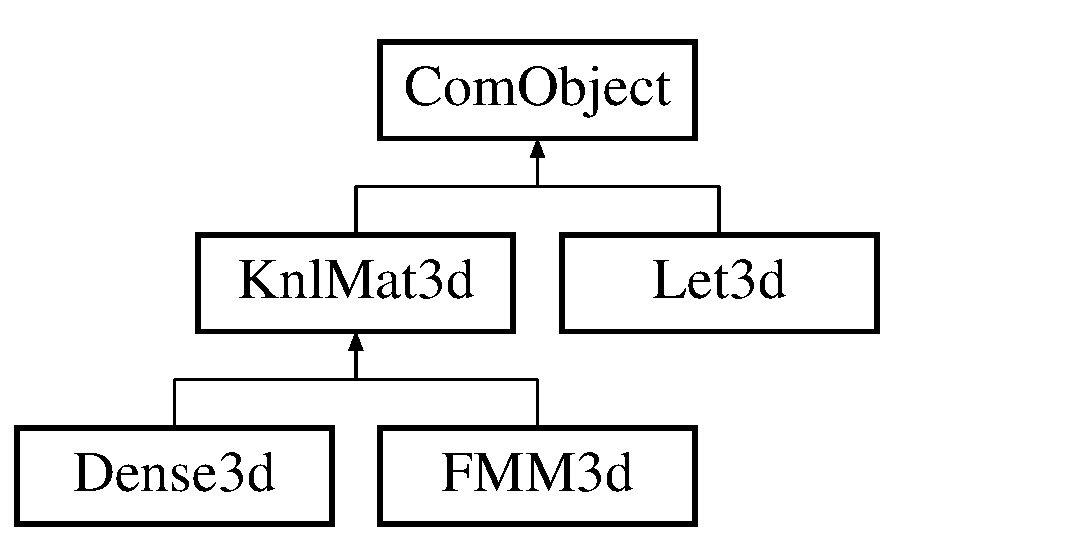
\includegraphics[height=3cm]{classComObject}
\end{center}
\end{figure}


\subsection{Detailed Description}
Com\-Object class for communication purposes. For sequential code, Com\-Object does very little. See comobject\_\-mpi.hpp for parallel code and how it is used $\ast$/. 



Definition at line 27 of file comobject.hpp.\subsection*{Public Member Functions}
\begin{CompactItemize}
\item 
{\bf Com\-Object} (const string \&prefix)
\item 
virtual {\bf $\sim$Com\-Object} ()
\item 
const string \& {\bf prefix} ()
\end{CompactItemize}
\subsection*{Protected Attributes}
\begin{CompactItemize}
\item 
string {\bf \_\-prefix}
\end{CompactItemize}


\subsection{Constructor \& Destructor Documentation}
\index{ComObject@{Com\-Object}!ComObject@{ComObject}}
\index{ComObject@{ComObject}!ComObject@{Com\-Object}}
\subsubsection{\setlength{\rightskip}{0pt plus 5cm}Com\-Object::Com\-Object (const string \& {\em prefix})\hspace{0.3cm}{\tt  [inline]}}\label{classComObject_cf233a08894f1cdd0f9bfb83b3251686_cf233a08894f1cdd0f9bfb83b3251686}


Initialize Com\-Object using string prefix 

Definition at line 34 of file comobject.hpp.

\footnotesize\begin{verbatim}34 : _prefix(prefix) {;}
\end{verbatim}\normalsize 


\index{ComObject@{Com\-Object}!~ComObject@{$\sim$ComObject}}
\index{~ComObject@{$\sim$ComObject}!ComObject@{Com\-Object}}
\subsubsection{\setlength{\rightskip}{0pt plus 5cm}virtual Com\-Object::$\sim$Com\-Object ()\hspace{0.3cm}{\tt  [inline, virtual]}}\label{classComObject_cf63f06cbc455a408453fe3d9d3dea0a_cf63f06cbc455a408453fe3d9d3dea0a}


Destroy Com\-Object 

Definition at line 36 of file comobject.hpp.

\footnotesize\begin{verbatim}36 {;}
\end{verbatim}\normalsize 




\subsection{Member Function Documentation}
\index{ComObject@{Com\-Object}!prefix@{prefix}}
\index{prefix@{prefix}!ComObject@{Com\-Object}}
\subsubsection{\setlength{\rightskip}{0pt plus 5cm}const string\& Com\-Object::prefix ()\hspace{0.3cm}{\tt  [inline]}}\label{classComObject_8171d0694121d77c4bfba18e5745faa9_8171d0694121d77c4bfba18e5745faa9}


Return \_\-prefic string 

Definition at line 39 of file comobject.hpp.

References \_\-prefix.

Referenced by Let3d::setup(), and FMM3d::setup().

\footnotesize\begin{verbatim}39 { return _prefix; }  
\end{verbatim}\normalsize 




\subsection{Member Data Documentation}
\index{ComObject@{Com\-Object}!_prefix@{\_\-prefix}}
\index{_prefix@{\_\-prefix}!ComObject@{Com\-Object}}
\subsubsection{\setlength{\rightskip}{0pt plus 5cm}string {\bf Com\-Object::\_\-prefix}\hspace{0.3cm}{\tt  [protected]}}\label{classComObject_b933f996cea3f524cf1514eb8539edfa_b933f996cea3f524cf1514eb8539edfa}


\_\-prefix is a string such as \char`\"{}fmm3d\_\-\char`\"{} which describes the type of object this is 

Definition at line 31 of file comobject.hpp.

Referenced by prefix().

The documentation for this class was generated from the following file:\begin{CompactItemize}
\item 
fmm3d/{\bf comobject.hpp}\end{CompactItemize}
